\chapter{Introduction}
\label{sec:introduction}

\vbox{
\centering

\includegraphics{satelliteicon}
\vspace{1cm}
}

BKNR is a software launch platform for Lisp satellites. You could
replace ``launch platform'' with framework and ``satellites'' with
``applications'', but that would be too many buzzwords.

BKNR is made of facilities that are not very useful on their own, but
they can be used to quickly build shiny and elegant Lisp
satellites. For example, a very important component of BKNR is its
datastore, which brings persistence to CLOS in a very simple way. By
adding a few declarations to your class definitions, you can have
persistent objects. You can also add XML import/export to your objects
in a similar way. I think this is the single most attractive feature
of BKNR: no more mapping from a relational database to Lisp objects,
no more XML parsing and XML generation, you just write plain
application code.


Another interesting feature of BKNR is its web framework, built on top
of the Hunchentoot webserver. The web framework has a simple
object-oriented handler hierarchy, with sessions, authorization and
all the features you are used to from other frameworks. It also
gathers usage information, stores it in the datastore, generates
statistics, maps sessions to persistent users. Furthermore, a very
useful feature is the HTML templater, which enables you to call Lisp
code from XML templates. The Lisp template callbacks are simple Lisp
functions that can work on the XML DOM representation. This eases
working with web developers, who can still use their standard editors
to develop the layout of the webpage. Dynamic content is easy to
integrate.

\begin{figure}[htbp]
    \centering
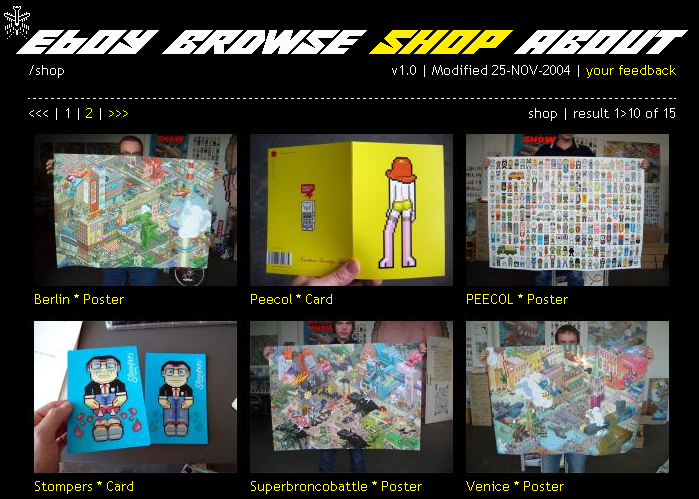
\includegraphics[scale=0.4]{eboyshot1}
\caption{Screenshot of eboy.com}
\end{figure}

The application which started BKNR was the website for the graphic
designers eboy. A lot of work went into the manipulation of images and
the integration of images into the Lisp framework. So another big part
of the BKNR web framework is the image manipulation code and the image
layout code, based on the CL-GD library by Edi Weitz.

We have started developing BKNR in March 2004, and it is used in 2 big
web applications (the Eboy dynasite ``eboy.com'', and the BOS website
``BOS creates rainforest''), and has been used to implement a few
personal websites (the website for the hacker gathering GPN in 2004,
which featured an interactive Lisp music-dj, the temporary conference
website for the European Lisp Workshop and the BKNR website). The code
was opensourced right from the start, but we didn't put a lot of
effort into making it accessible for other developers. This is the
first try at releasing some kind of public version of the BKNR
codebase, with (we hope) decent documentation.

If you would like to look at some of the BKNR features in a little
more detail, take the guided tour in Chapter 2. Chapters 3, 4, 5, 6
then show how to use the different facilities in short tutorials,
respectively object indices, the datastore, the web framework and the
templater. These chapters are slightly modified versions of the
tutorials that can be found in each of the facilities. Finally,
Chapter 7 shows how to build a full web photo album application using
BKNR. Due to time constraints, the last three chapters are not
available for the release of BKNR Sputnik. We are sorry for the
inconvenience. The sourcecode is in a working state, but not
documented and cleaned up yet.

We would like to thank the eboys for their support while developing
BKNR, their cool graphics and their enthusiasm :) We would also like
to thank Edi Weitz for his impressive libraries, and his
support. Also, I would like to thank Steffen Hurrle for his cool
website designs (he also has a new design for the BKNR website, which
sadly nobody has the time to update). The BKNR developers are Hans
Huebner, David Lichteblau and Manuel Odendahl.

